\section{The Fully-Hadronic Channel}\label{sec:dihad}

The large branching ratio of $\tau\tau \to \tau_{h}\tau_{h}$ (about 42\%) makes the contribution of the \ditauhad ~channel to the sensitivity of the overall analysis highly important. Because of the resemblance of QCD jets with $\tau_{h}$, the probability of misidentifying a QCD jet as a $\tau_{h}$ is at least an order of magnitude higher than that for a QCD jet to be misidentified as an electron or a muon. As a result, the final state is highly contaminated by QCD multijet background ($> 90\%$ of the background in the signal region). But, typical signal events are expected to appear at fairly high invariant mass values, where the QCD multijet contribution is strongly reduced owing to its rapidly falling production cross-section versus $\sqrt{s}$. Thus QCD multijet background only moderately affects the sensitivity of the analysis. Apart from QCD multijets, the other prevailing background is Drell-Yan processes giving rise to $\tau$ leptons. 

Similarly to other channels, the selections---designed to discriminate between the signal and background---are divided into: kinematic and geometric acceptance for selecting $\tau_{h}\tau_{h}$ pairs, $\tau_{h}$ identification, and topological selections. The main difference with the analyses of the $e\mu$, $\mu \tau_h$ and $e \tau_h$ channels are the substantially tighter $p_{T}(\tau_{h})$ requirements in order to stay efficient with respect to the trigger and targeting at the suppression of QCD multijet backgrounds (the exact selections are described below). Note that surviving pairs of $\tau_{h}$ candidates are preserved at each intermediate stage in the selections. In events in which more than one pair of unique $\tau_{h}$ candidates passes all the selections, only that pair with the highest $m(\tau_{h},\tau_{h},\MET)$ is selected. This requirement has a very high efficiency for both signal and backgrounds (the fraction of events with more than one pair is $\ll 1$\%).

Events fired by the $HLT\_DoubleMediumIsoPFTau35\_Trk1*$ trigger are considered as the interesting events for offline analysis. Events are required to have at 
least 2 HPS taus with $p_{T}$ greater than 60 GeV. These taus are required to have pseudorapidity value of $|\eta| < 2.1$. A $\tau_{h}$ candidate is also 
required to satisfy the the reconstruction and identification criteria described in section~\ref{sec:recoID}. The $\tau_{h}$ candidates are required to pass the 
following discriminators : ``DecayModeFindingNewDMs," ``TightCombinedIsoDB3Hits," ``againstMuonTight3,"  and ``againstElectronLooseMVA5."  The efficiency of 
these discriminators is shown in section~\ref{sec:tauIDeff}. These discriminators ensure the proper identification of a $\tau_{h}$ against QCD jets, muons and electrons. The candidate $\tau_{h}\tau_{h}$ pairs are required to be separated in $\eta-\phi$ space by $\Delta R(\tau_{h},\tau_{h}) > 0.3 $. Further, to reduce top pair contamination the event is required not to have any jet identified as a b-quark jet by the b–tagging algorithms using the “combined secondary vertex loose” (CSVL) working point. Further, each event must have at least 30 GeV of missing transverse energy to account for the neutrinos present in signal and further discriminate against the QCD multijet background. For consistency with the other channels, only 1- and 3-prong taus are considered. 

The $\tau_{h}\tau_{h}$ pair is expected to be back-to-back with $\cos(\delta\phi(\tau_{h},\tau_{h})) < -0.95$ . In addition, a ``$\zeta$" cut is used 
$(p_{\zeta}- 3.1\cdot p_{\zeta}^{vis} > -50)$ which is explained in Section \ref{sec:muTauhad}. These are topological cuts which reduce the contamination of backgrounds mainly from  $t\bar{t}$ and W+Jets processes to negligible levels.  



\subsection{QCD Background Estimation $\&$ Validation Strategy}

The main background for $\tau_{h}\tau_{h}$ final state is QCD multijet events ($>90\%$) and evaluated by a data-driven approach as a MC program does not model the background properly, nor does it provide sufficient statistics to make any strong conclusions.
%As already discussed, QCD is the main background of this final state. For its estimation, we rely on data-driven approach as MC statistics in not sufficient to model it properly.
The number of events in the signal region is given by the following equation: 

\begin{equation}                                                                                                                                                      
N_{\textrm{Signal}}^{\textrm{QCD}} = N_{\textrm{LS}}^{\textrm{QCD}} \cdot R_{OS/LS}
\end{equation}
   
Here $N_{\textrm{LS}}^{\textrm{QCD}}$ and $R_{OS/LS}$ are evaluated using the following approach. For its estimation, we rely on the classical method of counting events selected in a similar way to the signal events, but selecting $\tau_{h}\tau_{h}$ pairs with like-sign electrical charge. This criterion leads to events heavily dominated by the QCD multi-jet background. Assuming that QCD dijets are charge-blind, the number of like-sign events $N_{LS}$ should be equal to the number of opposite-sign $N_{OS}$ QCD multi-jet events after correcting $N_{LS}$ measured in data for known contamination from electroweak backgrounds using simulation. However, the assumption of the charge symmetry in events with two jets is not always true. An asymmetry in the charges of jets in multi-jet events can arise from the remaining correlation
between the quark charge and the leading track charge of the jet in events where quark charges are correlated. 
%e.g. $gg \to q \bar{q}$, $W \to q \bar{q}^{\prime}$. 
Note that the correlation between the charge of the quark and the charge of the track
becomes stronger in jets, in which the entire jet fluctuates into just a few high momentum tracks. Calculation of QCD $N_{LS}$ and $N_{OS}$ terms are made in control regions of the lower $\MET$ sidebands for the calculation of the asymmetry factor $R_{OS/LS}$ (shown in the next section). 
The contamination from signal in the LS control regions are small since the charge mis-measurement is small ($\sim 1-5\%$) for $m(Z^{\prime}) < 2.5$ TeV. 

The QCD estimation and validation strategy used in this analysis is shown in Figure~\ref{fig:qcd}. The shape is taken from region C and scaled to the signal estimation using a OS/LS scale factor derived in the low-$\MET$ sideband (regions B and D).    

 \begin{figure}[tbh!]
     \centering
     \begin{tabular}{cc}
       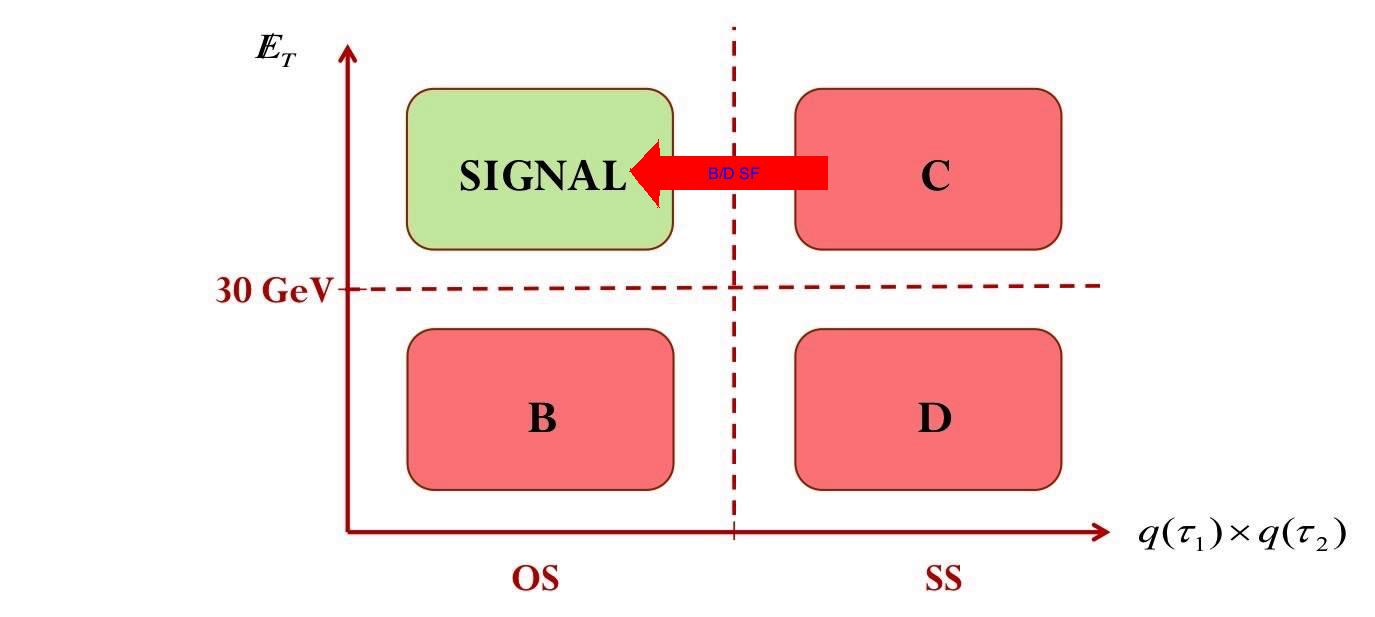
\includegraphics[width=0.75\textwidth]{figures/QCD_Strategy.jpg}
     \end{tabular}
     \caption{QCD estimation and validation strategy for the $\tau_{h}\tau_{h}$ channel.}
    \label{fig:qcd}
   \end{figure}


The shape of the $m(\tau_{h},\tau_{h},\MET)$ distribution is obtained from control region C (same-sign $\tau_{h}\tau_{h}$ with nominal $\MET$). To extract the OS/LS ratio from data, two control regions, B and D, are obtained by keeping the same selections as signal selections, but inverting the $\MET$ cut $(\MET < 30$ GeV) and requiring OS and LS $\tau_{h}\tau_{h}$ pairs respectively. The contribution of non-QCD MC backgrounds (Drell-Yan + Jets, $t\bar{t}$, W + Jets, and diboson) are subtracted from data in these control regions and then the $R_{OS/LS}$ is measured:

\begin{center}
\begin{eqnarray}
 N^{\textrm{QCD}}_{\textrm{OS}} = N^{\textrm{Data}}_{\textrm{OS}} - N^{\textrm{non-QCD MC}}_{\textrm{OS}} \nonumber\\
 N^{\textrm{QCD}}_{\textrm{LS}} = N^{\textrm{Data}}_{\textrm{LS}} - N^{\textrm{non-QCD MC}}_{\textrm{LS}} \\  
% R_{\textrm{OS/LS}} = QCD_{\textrm{OS}}/QCD_{\textrm{LS}} \nonumber\\ 
R_{\textrm{OS/LS}} = N^{\textrm{QCD}}_{\textrm{OS}}/N^{\textrm{QCD}}_{\textrm{LS}} \nonumber\\ 
\label{eqn:OSLSratio}
\end{eqnarray}
\end{center}

Table~\ref{table:OLSStable} shows the data and MC yields in controls regions B and D. The purity of QCD multijet, defined by Data - $\sum\limits_{i} BG_{i}$, is 
approximately $96-99$\% depending on the sample. The measured OS/LS ratio is $1.64\pm0.21$. The above equation shows the mathematical procedure used to obtain 
this ratio. 

Closure and validation tests for the background estimation method outlined above is performed with real data, since there are insufficient statistics to perform 
such a test with simulation. Two aspects are simultaneously tested: (1) closure on the normalization (i.e. $N_{\textrm{QCD}}^{A} = N_{\textrm{QCD}}^{C} \cdot 
\frac{N_{\textrm{QCD}}^{B}}{N_{\textrm{QCD}}^{D}}$); (2) correct determination of the $m(\tau_{h},\tau_{h},\MET)$ shape. In order to check (with data) whether same-sign $\tau_{h}\tau_{h}$ events can correctly model the mass shapes in the opposite-sign regions, we perform a shape closure/validation test by taking the shape from region D (obtained as Data - $\sum\limits_{i} BG_{i}$) and normalize it to the QCD yield in control region B. By comparing the
shape for the QCD prediction in region B with the observed mass spectrum in the same region, we can determine whether same-sign $\tau_{h}\tau_{h}$ correctly models the mass shapes in the opposite-sign region. Furthermore, any disagreement in the shape between data and the QCD prediction can be used to assign systematic uncertainty on the shape. Figure~\ref{fig:MG304} shows the $m(\tau_{h},\tau_{h},\MET)$ mass distribution for this closure test in control region B. We observe very good agreement between the observed shape and the predicted shape and thus no additional
systematic uncertainties are applied due to this particular closure test on the shape. 



\begin{table}[!htpb]
   \caption{ Yields in the control regions B and D used for calculation of OS/LS ratio.}
   \centering{
     \begin{tabular}{ | l | c | c | }
        \hline \hline
        Process & OS $\tau_{h}\tau_{h}$ isolated + MET $<$ 30 GeV  & SS $\tau_{h}\tau_{h}$ isolated + MET $<$ 30 GeV \\ \hline
        Data & 207 & 113 \\ \hline
        W + Jets & 0.897455 $\pm$ 1.57954 & 1.20229 $\pm$ 1.26803 \\ \hline
        Z + Jets & 21.8385 $\pm$ 4.67317 & 0.132112 $\pm$ 0.363472 \\ \hline
        WZ + Jets & 0 $\pm$ 0 & 0 $\pm$ 0 \\ \hline
        WW + Jets & 0.522162 $\pm$ 0.800846 & 0 $\pm$ 0 \\ \hline
        ZZ + Jets & 0.0522376 $\pm$ 0.232475 & 0 $\pm$ 0 \\ \hline
        $t\bar{t}$ & 0.0111017 $\pm$ 0.112979 & 0 $\pm$ 0 \\ \hline
        Data - $\sum\limits_{i} BG_{i}$ & 183.679 $\pm$ 15.2329 & 111.666 $\pm$ 10.7117 \\ \hline \hline
        OS/LS ratio       &$1.64\pm0.208$     & \\ \hline \hline
     \end{tabular}




   }
   \label{table:OLSStable} % is used to refer this table in the text
 \end{table}
  
\begin{figure}[tbhp!]
      \centering
      \begin{tabular}{cc}
        \includegraphics[width=0.45\textwidth]{figures/OSLowMetCR_NormalScale_1or3prong.png}
        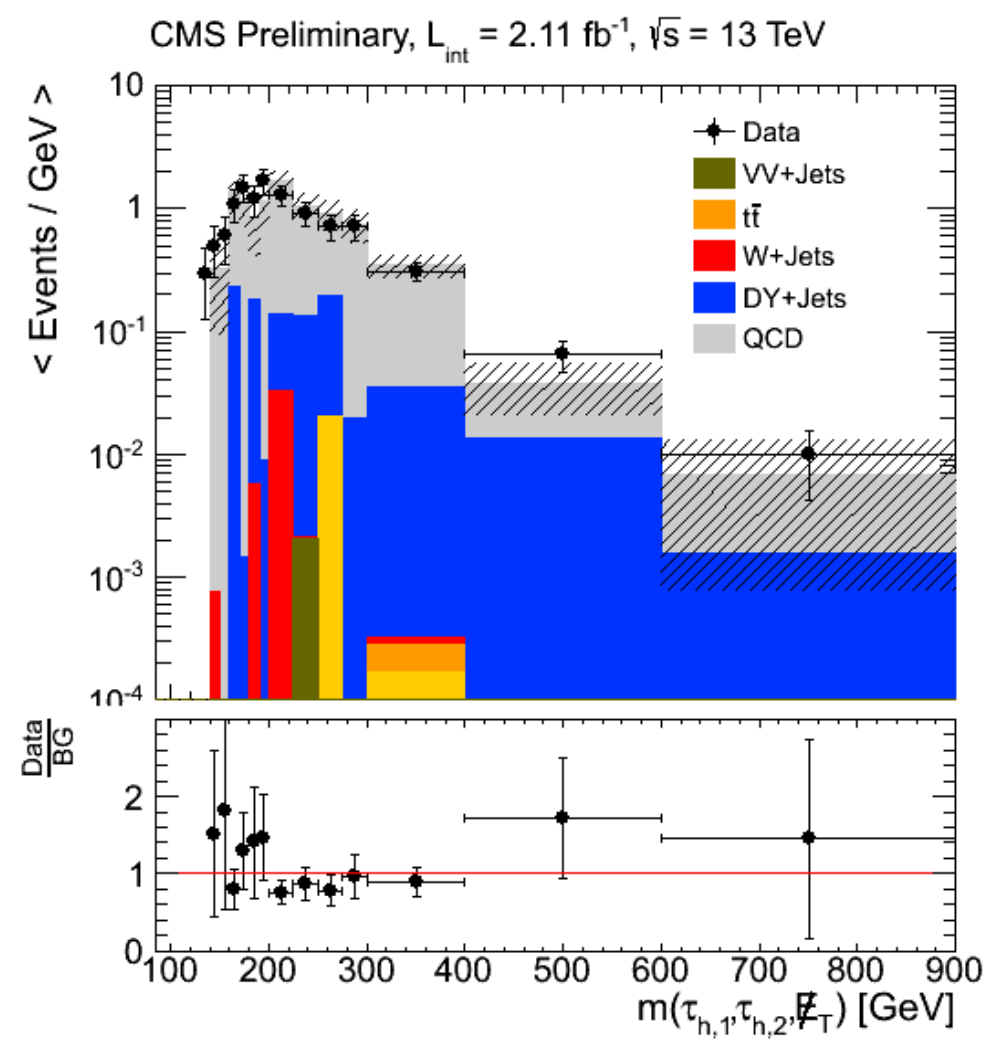
\includegraphics[width=0.45\textwidth]{figures/OSLowMetCR_LogScale_1or3prong.png}
      \end{tabular}
     \caption{$\tau_{h} - \tau_{h}$ mass distribution in isolated OS, low-$\MET$ sideband (region B). Left: normal scale.  Right: log scale.}
    \label{fig:MG304}
 \end{figure}

\begin{figure}[tbhp!]
      \centering
      \begin{tabular}{cc}
        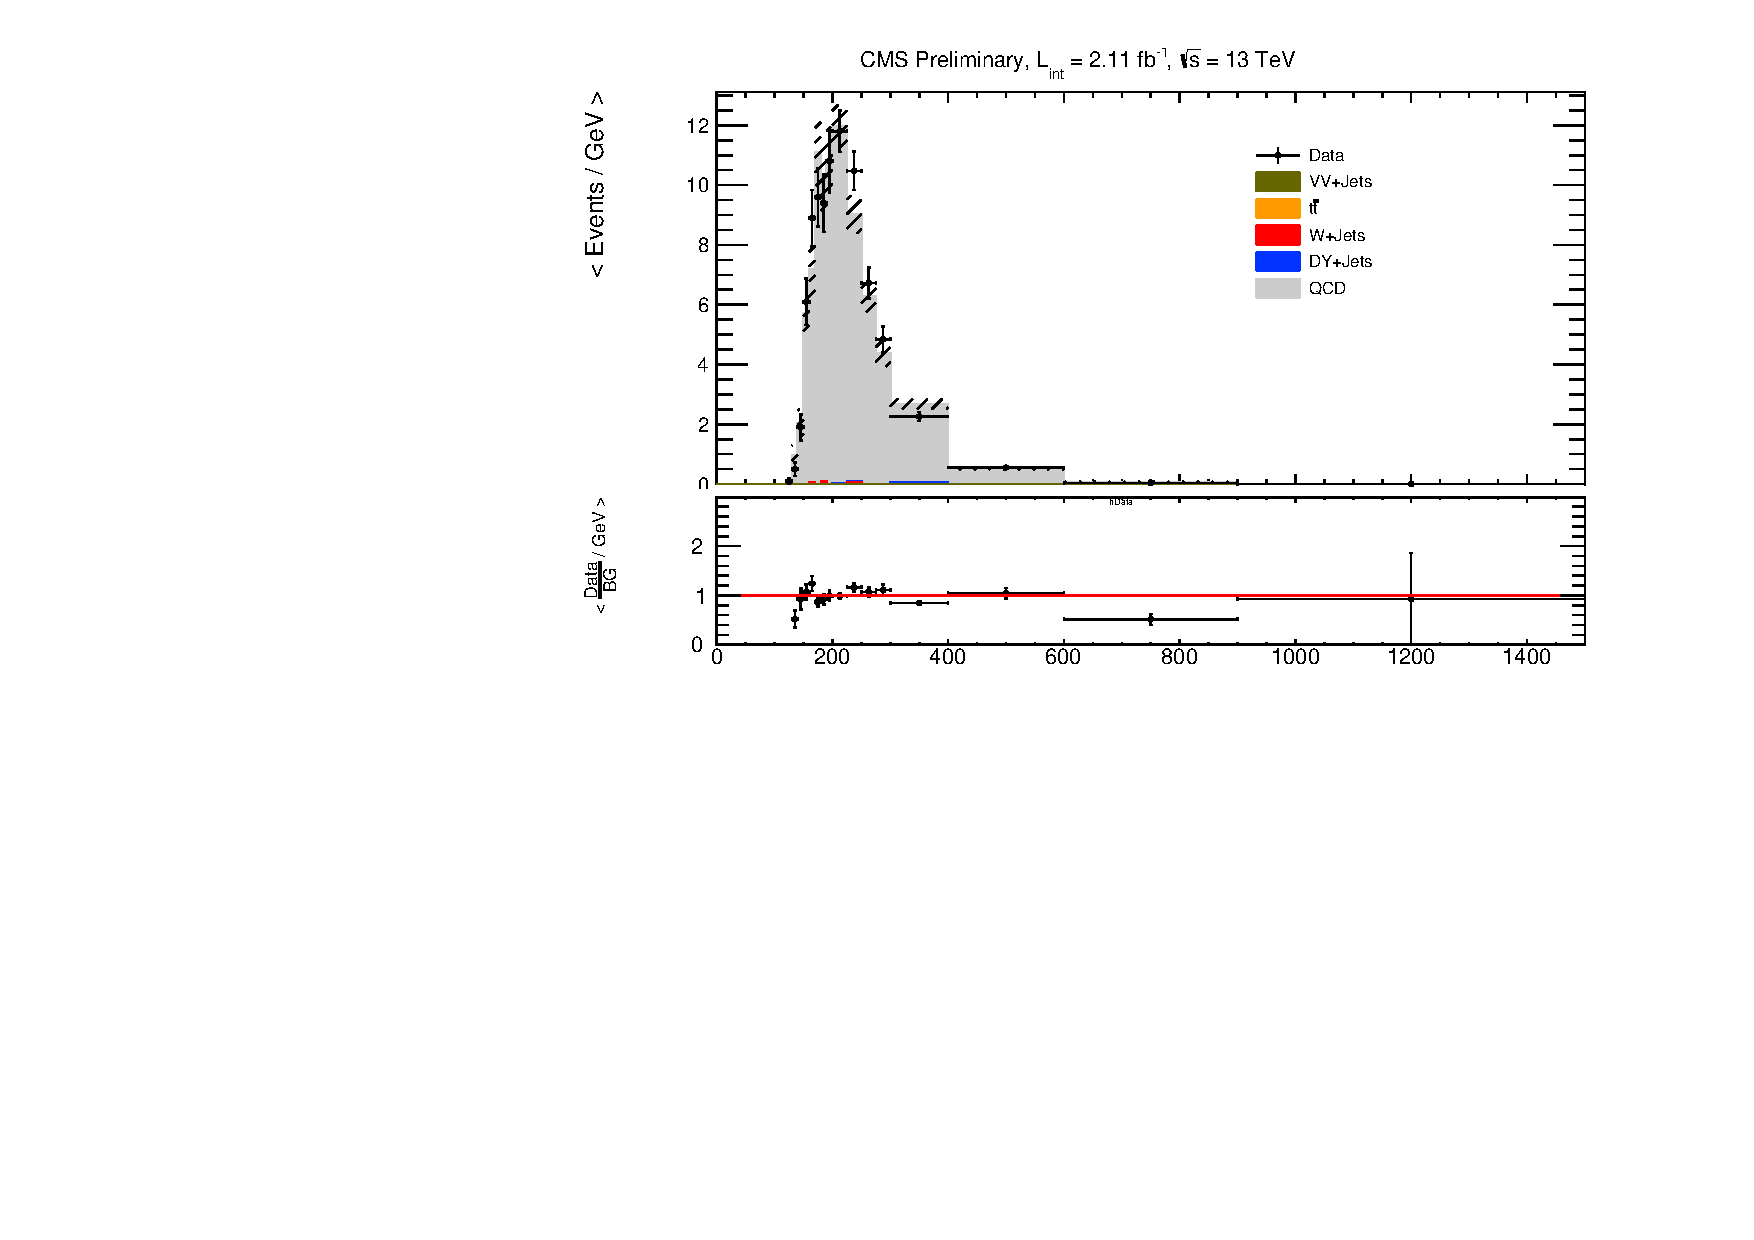
\includegraphics[width=0.45\textwidth]{figures/QCDBGEst_Closure_LowMET_CR_1_20_16.pdf}
        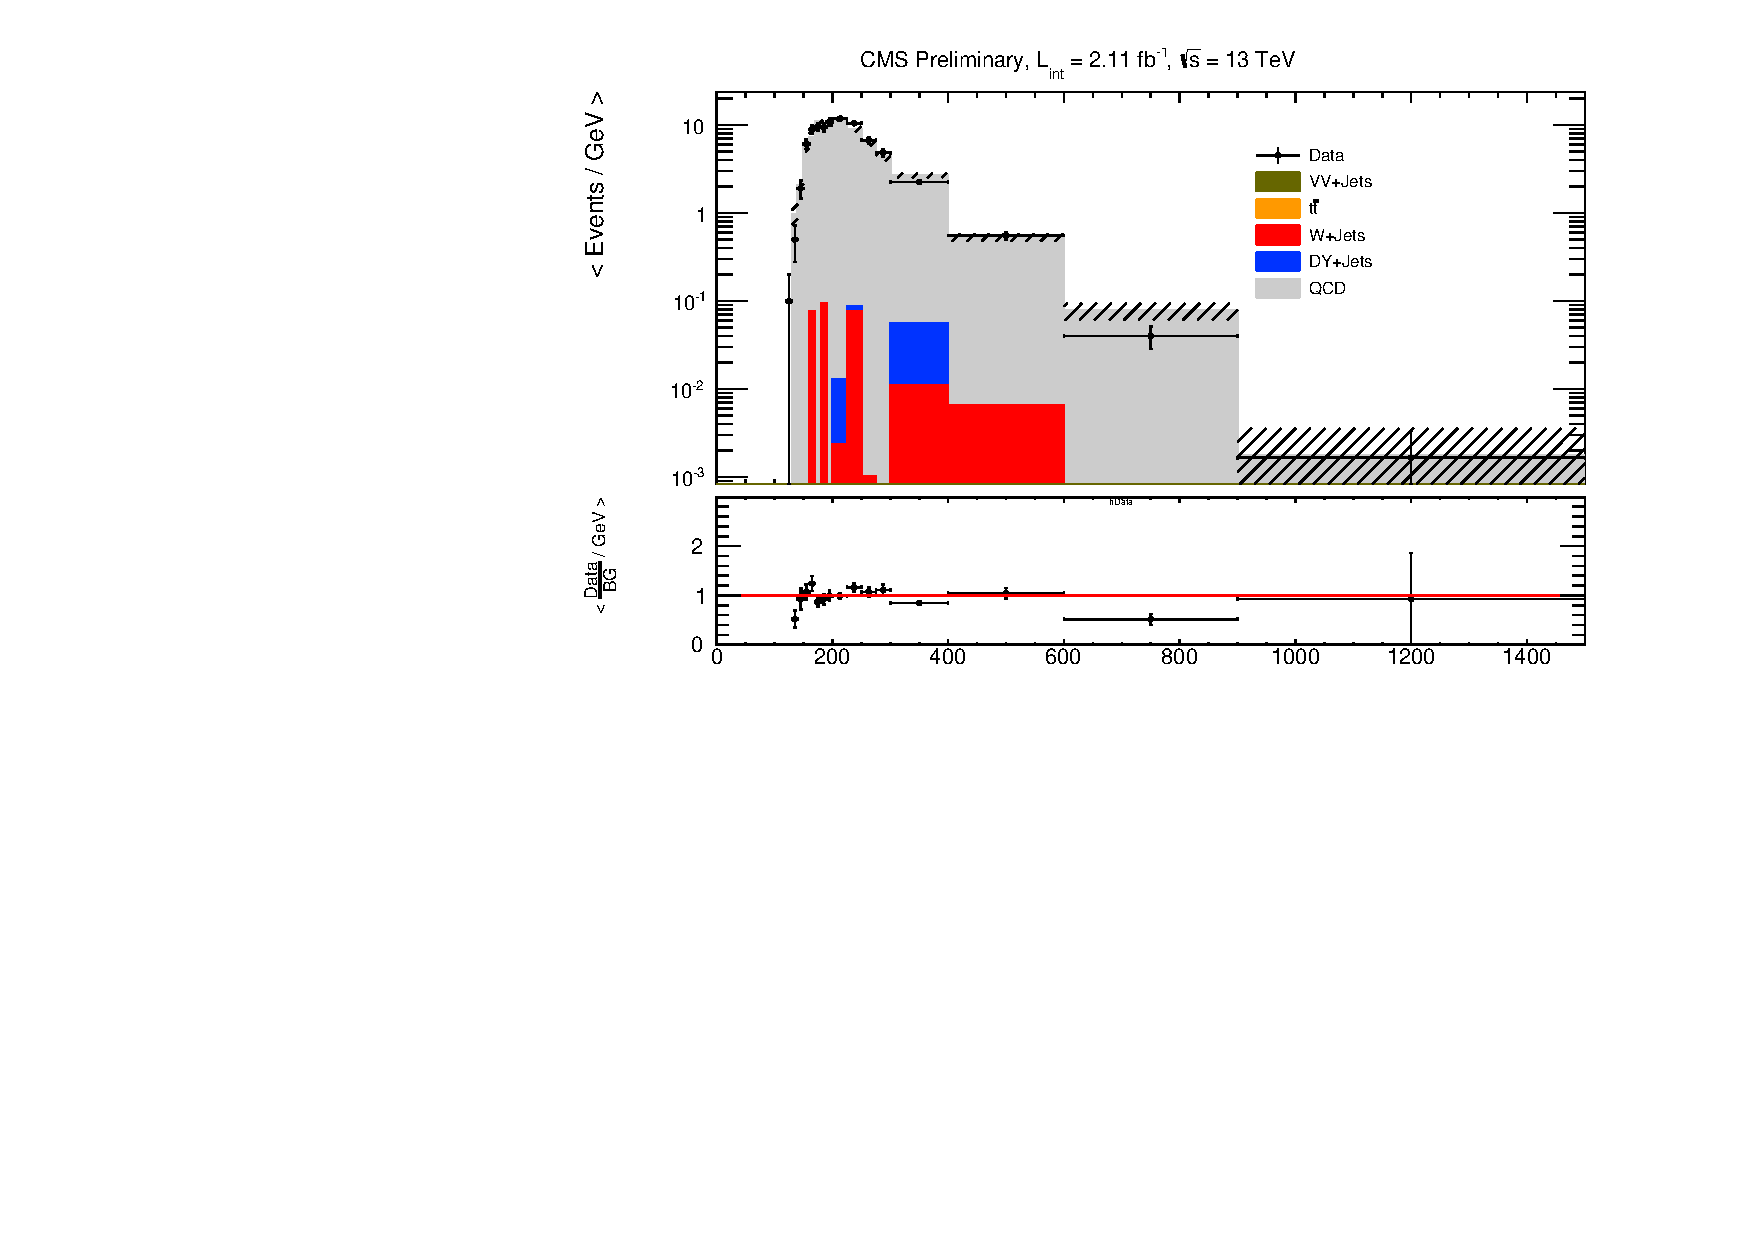
\includegraphics[width=0.45\textwidth]{figures/QCDBGEst_Closure_LowMET_CR__Log_1_20_16.pdf}
      \end{tabular}
     \caption{$m(\tau_{h},\tau_{h},\MET)$ mass distribution in anti-isolated OS, low-$\MET$ sideband (region 2B) Left: normal scale.  Right: log scale.}
    \label{fig:MG305}
 \end{figure}


Two additional control samples are utilized in order to provide further closure for this method. Control regions 2B and 2D are obtained by using
the $\tau_{h}$ anti-isolation sidebands (passing the ``loose" isolation working point and failing the ``tight" isolation working point) with otherwise similar selections
to control regions B and D (low $\MET$). The QCD multi-jet prediction in control region 2B is determined as data minus non-QCD backgrounds. The QCD shapes and 
rates extracted from control region 2D (after subtracting non-QCD backgrounds) are normalized to the QCD yield in control region 2B. Figure ~\ref{fig:MG305} 
summarizes this closure test. Nice agreement between the data and predicted QCD rate in control region 2B (Figure ~\ref{fig:MG305}) validates the
ability to extract the shapes of distributions in OS from LS samples (we will extract the QCD signal region $m(\tau_{h,1},\tau_{h,2},\MET)$ shape from LS data).
%To validate the measured OS/LS ratio with the data itself, two additional control samples are utilized, 2B and 2D. Control regions 2B and 2D are obtained by using 
%the $\tau_{h}$ isolation sidebands (passing the "loose" isolation working point and failing the "tight" isolation working point) with otherwise similar selections 
%to control regions 1B and 1D (low $\MET$). To determine the QCD multi-jet prediction in control region 2B, the QCD shapes and rates extracted from control region 
%2D (after subtracting non-QCD backgrounds) are scaled by the OS/LS ratio obtained from control regions 1B and 1D. Figure ~\ref{fig:MG305} summarizes this closure 
%test. Nice agreement between the data and predicted QCD rate in control region 2B (Figure ~\ref{fig:MG305}) validates the measured OS/LS ratio as well as the 
%ability to extract the shapes of distributions in OS from LS samples (we will extract the QCD signal region $m(\tau_{h,1},\tau_{h,2},\MET)$ shape from LS data).  

Next we perform the full-blown closure test for the ABCD method by comparing the observed yield and mass spectrum in control region $2A$ (OS, non-isolated $\tau_{h}\tau_{h}$ with nominal $\MET$) with the QCD multijet prediction in that same region obtained by using the QCD shape from region $2C$ and normalizing it to $N_{\textrm{QCD}}^{2A} = N_{\textrm{QCD}}^{2C} \cdot \frac{N_{\textrm{QCD}}^{2B}}{N_{\textrm{QCD}}^{2D}}$. Figure~\ref{fig:MG306} shows the closure test in region $2A$, showing agreement between data and prediction. The QCD multijet prediction in control region 2A, using the ABCD method, is $427 \pm 26$, while the observed yield is $429$. Thus, no additional systematic uncertainties are applied due to closure.

%\begin{table}[!htpb]
%    \caption{ Events in the control regions 2B and 2D. }
%    \centering{
%     \begin{tabular}{| l | c | c |}
%        \hline\hline
%        Sample                    & Events (OS)                & Events (LS)         \\ [0.5ex] \hline
%        Data                      & $1669$                       & $1553$ \\
%        ${\rm W+Jets}$            & $6.09\pm2.84$                & $11.23\pm4.935$ \\
%        ${\rm Z+Jets}$            & $5.03\pm3.20$                & $1.29\pm1.20$ \\
%        ${\rm WZ+Jets}$            & $0\pm0$                & $0\pm0$ \\
%        ${\rm WW+Jets}$            & $0\pm0$                & $0\pm0$ \\
%        ${\rm ZZ+Jets}$            & $0.01\pm0.1$                & $0\pm0$ \\
%        $t \overline{t} $         & $0\pm0$                        & $0.133\pm0.393$ \\
%        \hline\hline
%        ${\rm Data - $\sum\limits_{i} BG_{i}}$      &$1657.87 \pm 41.0774$          & $1540.35 \pm 39.736 \\
%        \hline\hline         
%\end{tabular} 
%    }
%   \label{table:OLLStable2} % is used to refer this table in the text
% \end{table}


 \begin{figure}[tbhp!]
      \centering
      \begin{tabular}{cc}
        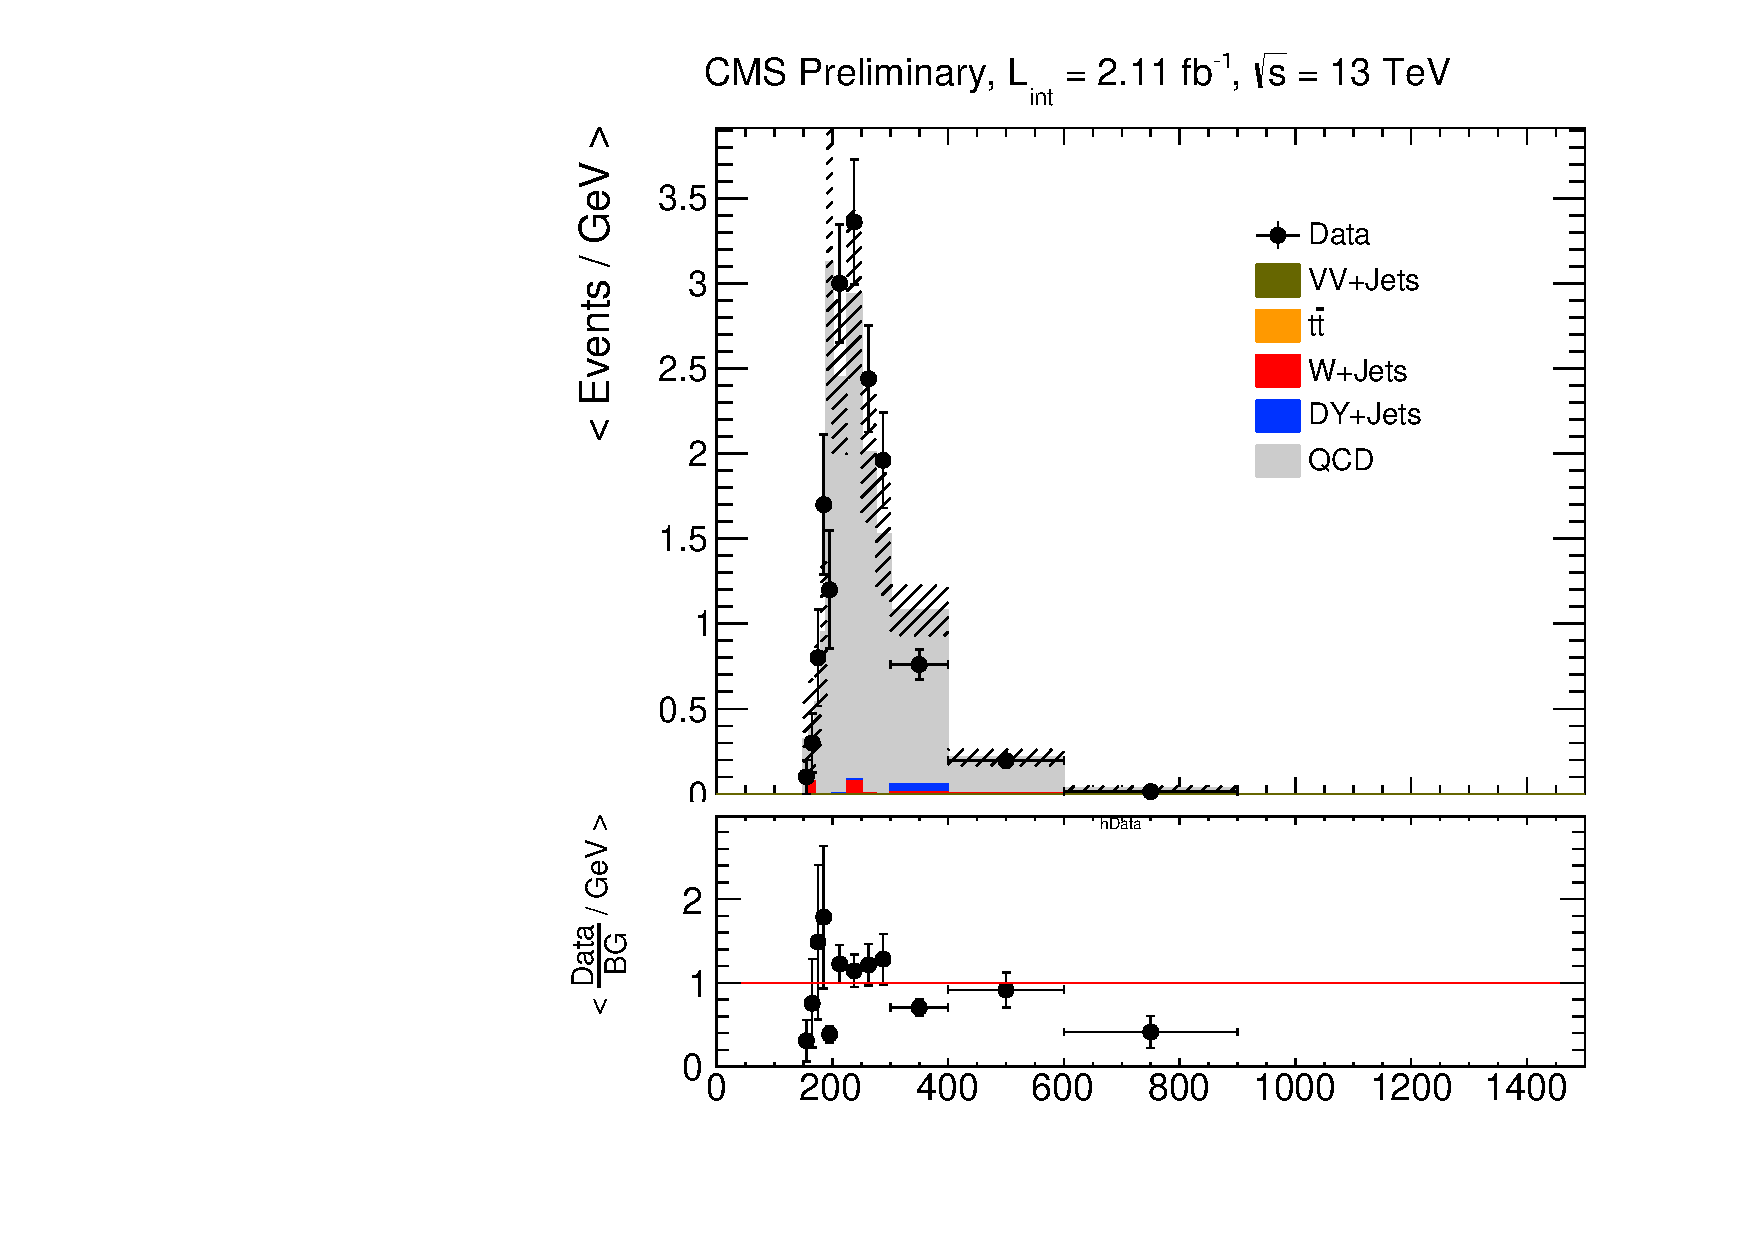
\includegraphics[width=0.45\textwidth]{figures/QCDBGEst_Closure_SR_1_20_16.pdf}
        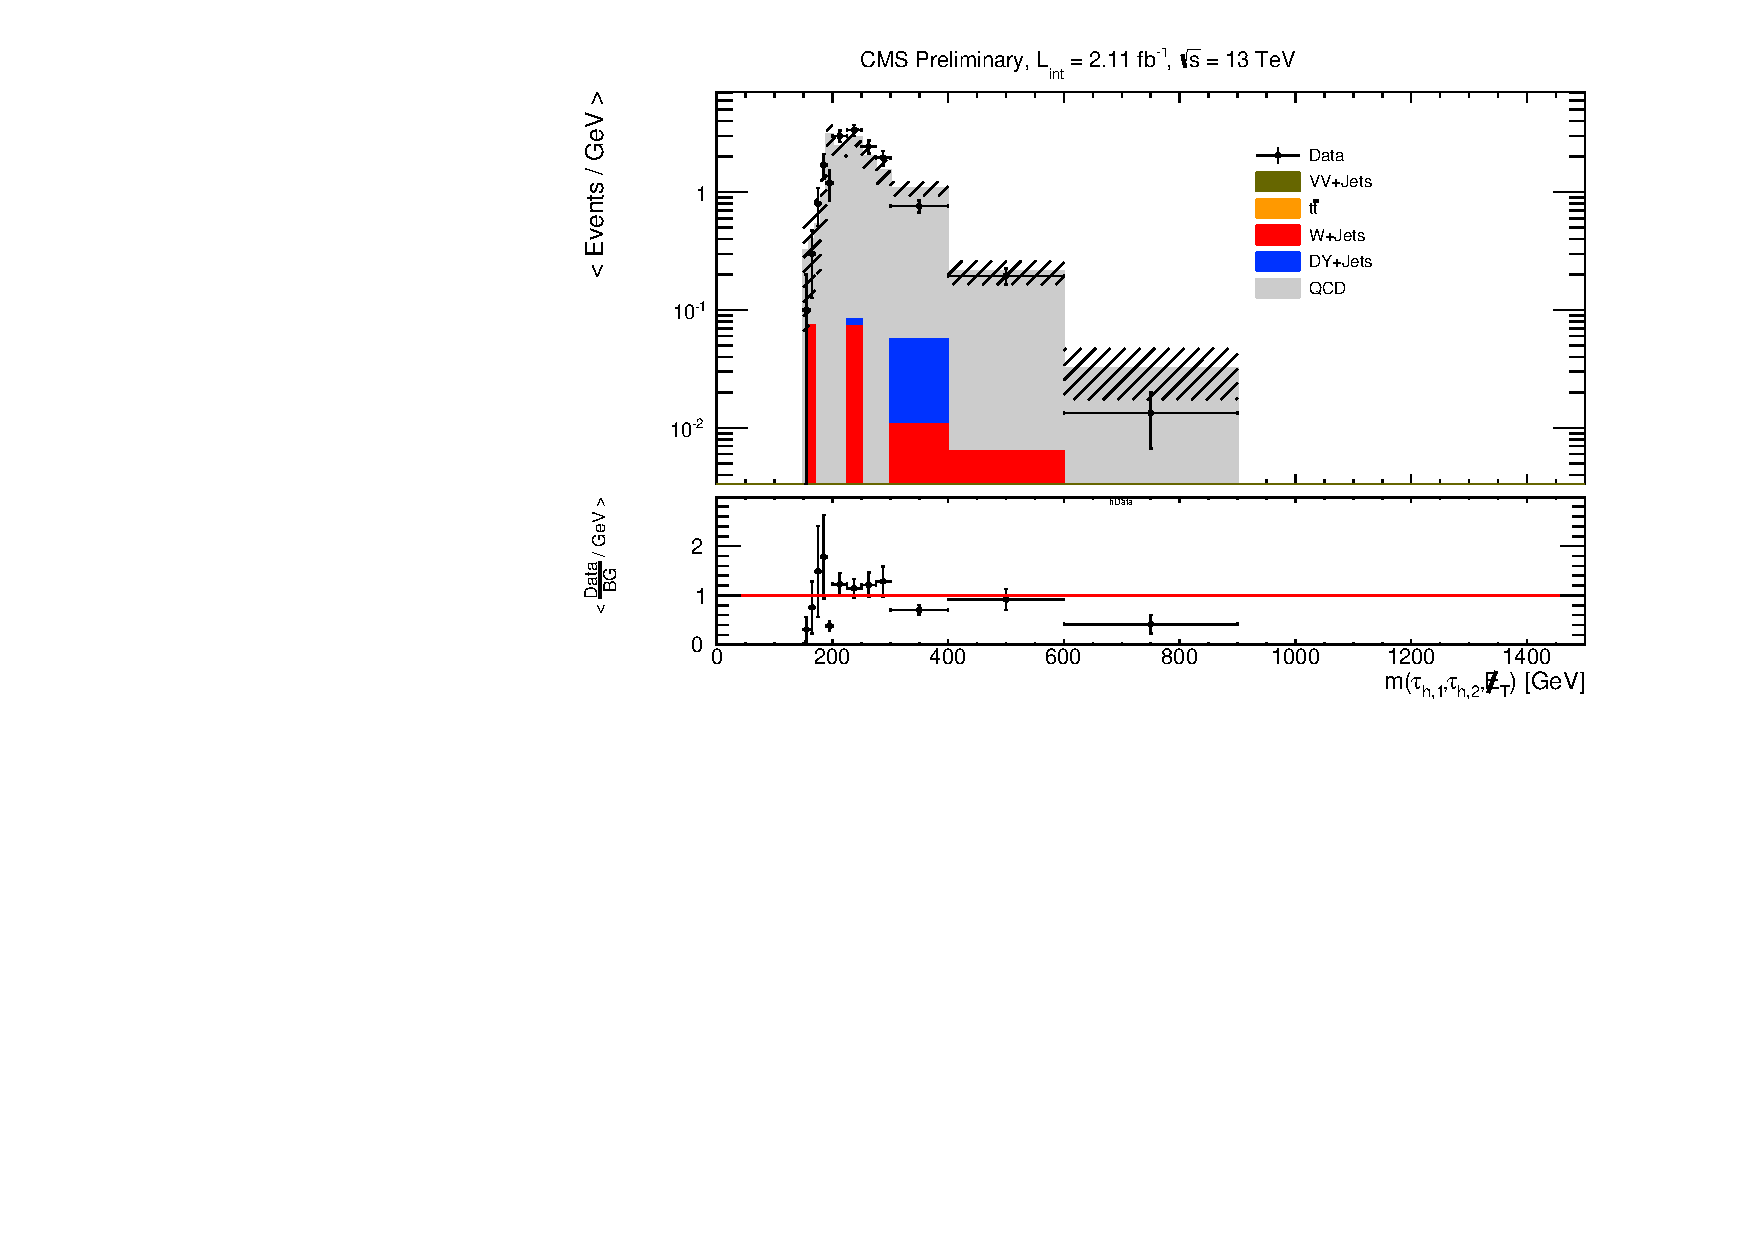
\includegraphics[width=0.70\textwidth]{figures/QCD_Closure_SR_FixedTitles_Log_1_26_16.pdf}
      \end{tabular}
     \caption{$m(\tau_{h},\tau_{h},\MET)$ mass distribution in anti-isolated OS region with nominal $\MET$ (Left: normal scale.  Right: log scale).}
    \label{fig:MG306}
 \end{figure}
 
         
Table \ref{tab:SignalEst} represents the event rate of data and backgrounds in regions A (signal region) and C (same-sign, isolated $\tau_{h}\tau_{h}$ with nominal $\MET$). QCD 
shapes/rates are extracted in data-driven way from control region C and scaled by the OS/LS ratio determined from control region B and D. The non-QCD 
backgrounds are taken directly from MC in Table \ref{tab:SignalEst} (see the next section for a validation of the DY + Jets background yield). Other processes such as W + Jets, 
$t\bar{t}$, and diboson represent only $\sim 1$\% of the total background 
rate in the signal region, and are thus taken directly from MC. The final prediction of QCD events in the signal region A is given in the right-most column of 
Table \ref{tab:QCDBGEstimationTable}. The procedure outlined in this section yields a QCD estimate of $N_{\textrm{QCD}}^{\textrm{Signal}} = 48.7 \pm 11.0$. The uncertainty is based on the 
statistics of the data and MC samples. We stress that this is the QCD predicted rate over the entire $m(\tau_{h},\tau_{h},\MET)$ spectrum. As was mentioned
in the strategy section of this note, we fit for a potential signal that would appear as an excess of events over the standard model expectation in the high 
$m(\tau_{h},\tau_{h},\MET)$ part of the distribution. The total predicted background $m(\tau_{h},\tau_{h},\MET)$ spectrum will be shown in the results section of 
this chapter. 

\begin{table}[htbp!]
  \centering{
  \caption{Background and data yields in QCD control regions $A$ and $C$ under nominal isolation and $\MET$ conditions (i.e. isolated $+$ $\MET > 30$ GeV).}  \label{tab:SignalEst}

\begin{tabular}{ | l | c | c | }
\hline \hline
Process & OS $\tau_{h}\tau_{h}$ isolated + MET $>$ 30 GeV  & SS $\tau_{h}\tau_{h}$ isolated + MET $>$ 30 GeV \\ \hline
Data & 55 & 30 \\ \hline
W + Jets & 0.09 $\pm$ 0.35 & 0.28 $\pm$ 0.61 \\ \hline
Z + Jets & 8.1 $\pm$ 2.8 & 0.10 $\pm$ 0.32 \\ \hline
WZ + Jets & 0 $\pm$ 0 & 0 $\pm$ 0 \\ \hline
WW + Jets & 0.49 $\pm$ 0.77 & 0 $\pm$ 0 \\ \hline
ZZ + Jets & 0 $\pm$ 0 & 0 $\pm$ 0 \\ \hline
$t\bar{t}$ & 0 $\pm$ 0 & 0 $\pm$ 0 \\ \hline
Data - $\sum\limits_{i} BG_{i}$ & 46.3 $\pm$ 8.0 & 29.6 $\pm$ 5.5 \\ \hline \hline
\end{tabular}
  }

\end{table}

\begin{table}[htpb!]
  \centering{
  \caption{QCD yields in the isolated regions $A$ (signal region), $B$, $C$, and $D$.}  \label{tab:QCDBGEstimationTable}
  \scalebox{0.7}{

\begin{tabular}{ | l | c | c | c | c | }
\hline \hline
Region & OS $\tau_{h}\tau_{h}$ + MET $<$ 30 GeV  & SS $\tau_{h}\tau_{h}$ + MET $<$ 30 GeV  & SS $\tau_{h}\tau_{h}$ + MET $>$ 30 GeV  & OS $\tau_{h}\tau_{h}$ + MET $>$ 30 GeV \\ \hline
isolated & 183.7 $\pm$ 15.4 & 111.7 $\pm$ 10.7 & 29.6 $\pm$ 5.5 & 48.7 $\pm$ 11.0 \\ \hline \hline
\end{tabular}





  }
  }
\end{table}

